\section{Expansion of Model}
\subsection{Mathematical Model for Spread of Smoke and Gas}
In the real context, the smoke is also a significant contributing factor to the productivity of the firefighters. Giving the fact that the smoke and poisonous gas is keep spreading and cannot be approximated by a simple linear transport. A model based on \textbf{Navier-Stokes equations} was established, in order to better simulate the real circumstances. Governing equations are as follows:
\begin{equation}
\left\{
\begin{aligned}
&\nabla \cdot \mathbf{u} = 0 \\
&\frac{\partial \mathbf{u}}{\partial t} + (\mathbf{u} \cdot \nabla)\mathbf{u} = -\frac{1}{\rho_0}\nabla p + \nu \nabla^2 \mathbf{u} + \beta g (T - T_0)\mathbf{j} \\
&\frac{\partial T}{\partial t} + (\mathbf{u} \cdot \nabla)T = \kappa_T \nabla^2 T + S_T \\
&\frac{\partial C}{\partial t} + (\mathbf{u} \cdot \nabla)C = \kappa_C \nabla^2 C + S_C
\end{aligned}
\right.
\end{equation}

This mathematical model is based on incompressible flow with \textbf{Boussinesq approximation}, where: $\mathbf{u}$ is velocity vector, $p$ is pressure, $T$ is temperature, $C$ is smoke concentration, $\rho_0$ is reference density, $\nu$ is kinematic viscosity, $\beta$ is thermal expansion coefficient, $g$ is gravitational acceleration, $T_0$ is ambient temperature, $\mathbf{j}$ is vertical unit vector, $\kappa_T$ is thermal diffusivity, $\kappa_C$ is mass diffusivity, $S_T$ is heat source term, and $S_C$ is smoke source term. 

The coupled system describes \textbf{buoyancy-driven flow and scalar transport}, which is the continuity equation ensuring mass conservation; the momentum equation incorporates the temperature-induced density variations in the gravity term via Boussinesq approximation; the energy and concentration equations describe convective-diffusive transport; the velocity field simultaneously transports heat and smoke, while temperature variations drive fluid motion through buoyancy effects, forming a fully coupled physical system.

The governing partial differential equations are solved by \textbf{MATLAB 2021a} using the finite difference method combined with the fractional step projection algorithm. This numerical framework efficiently handles the strong coupling between fluid flow, temperature, and concentration fields in smoke transport simulations.


\begin{figure}[hbtp]
    \centering
    
\includegraphics[width=\textwidth]{smoke} % 替换为实际图片路径
    \caption{Smoke Concentration at Each Position Over Time}
    \label{smoke1}
\end{figure}


For the single-story office building with six rooms in Scenario 1, when the fire source is located in the upper-left corner room, the visualization of smoke spread over time is shown in Figure\ref{smoke1}. The three sub-figures from left to right correspond to the smoke distribution 1 minute, 2 minutes, and 10 minutes after the fire starts respectively.


\subsection{Discrete Smoke Diffusion Model Formulation}
It's undeniable that continuous partial differential equation systems can accurately describe physical processes, in smoke transport simulations within complex building environments, however, they may be difficult or impossible to solve, and demand too much computational resources. Discrete models, in contrast, could retain the key dynamic characteristics of smoke propagation while reducing computational complexity to an acceptable level.
\textbf{Model Discretization Strategy}

The continuous smoke diffusion model is discretized into a network-based representation where:
\begin{itemize}
    \item Rooms are represented as nodes $R_i \in \mathcal{R}$
    \item Pathways between rooms are represented as edges $E_{ij} \in \mathcal{E}$
    \item Smoke concentration evolves over discrete time steps $t_k = k\Delta t$
\end{itemize}

\textbf{Discrete Governing Equations}

Room concentration evolution: 
\[
C_i(t_{k+1}) = C_i(t_k) + \Delta t \left[ S_i(t_k) - \sum_{j \in \mathcal{N}(i)} F_{ij}(t_k) + D \sum_{j \in \mathcal{N}(i)} (C_j(t_k) - C_i(t_k)) \right]
\]

Pathway concentration evolution:
\[
C_{ij}(t_{k+1}) = \frac{1}{2} \left[ C_i(t_k) + C_j(t_k) \right] + \Delta t \left[ -v_{ij} \frac{C_j(t_k) - C_i(t_k)}{L_{ij}} + D \frac{C_j(t_k) - 2C_{ij}(t_k) + C_i(t_k)}{L_{ij}^2} \right]
\]

Flow between rooms:
\[
F_{ij}(t_k) = v_{ij} A_{ij} \cdot \text{sign}(P_j(t_k) - P_i(t_k)) \cdot \min(C_i(t_k), C_j(t_k))
\]

Pressure difference:
\[
P_i(t_k) = \alpha T_i(t_k) + \beta C_i(t_k)
\]

where \( C_i(t_k) \) denotes the average smoke concentration in room \( i \) at time \( t_k \); \( C_{ij}(t_k) \) is the average smoke concentration along pathway \( i \)-\( j \); \( S_i(t_k) \) represents the smoke source term in room \( i \); \( F_{ij}(t_k) \) is the smoke flow rate from room \( i \) to \( j \); \( v_{ij} \) is the characteristic flow velocity in pathway \( i \)-\( j \); \( D \) denotes the effective diffusion coefficient; \( L_{ij} \) is the length of pathway \( i \)-\( j \); and \( A_{ij} \) represents the cross-sectional area of pathway \( i \)-\( j \).


\begin{figure}[hbtp]
    \centering
    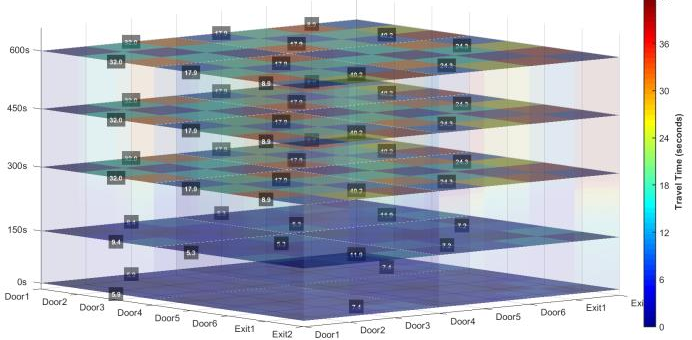
\includegraphics[width=\textwidth]{fig/travellingtime.png} % 替换为实际图片路径
    \caption{$T_move$ Heat Map Over Time}
    \label{heat}
\end{figure}


\subsection{Smoke Impact and Risk Assessment Models}

\subsubsection{Influence of Smoke Density on Sweeping Speed}

 Smoke reduces mobility by reducing visibility, causing physiological irritation, and inducing psychological panic.

\paragraph{Conversion Relationship Between Smoke Concentration and Optical Density}

In fire engineering, smoke concentration is typically expressed as mass concentration \( C \) , while evacuation behavior research commonly uses optical density or extinction coefficient \( C_s \) to quantify visibility. The conversion relationship between them is given by \upcite{Mulholl,1998}:

\begin{equation}
C_s = K_m \cdot C
\label{eq:conversion}
\end{equation}

Where:
\( C_s \) is the extinction coefficient (\si{\per\meter}),
\( C \) is the smoke mass concentration (\si{\gram\per\cubic\meter})
and \( K_m \) is the mass extinction coefficient (\si{\square\meter\per\gram}), with typical values ranging from \numrange{0.1}{1.0}

For smoke produced by common building materials, \( K_m \) can be taken as an average value of \SI{0.5}{\square\meter\per\gram}. In practical applications, an approximate inverse relationship exists between the extinction coefficient \( C_s \) and visibility \( V \) (unit: \si{\meter}):
\begin{equation}
V \approx \frac{3}{C_s}
\label{eq:visibility}
\end{equation}







\paragraph{Quantitative Relationship Between Sweeping Time and Smoke Density}

As the concentration of smoke in the room increase, the visibility of firefighter would decrease. We assume the time required to sweep a room thoroughly obey a liner relationship with $C_s$, meaning that $$T_s \propto C_s $$ where $T_S$ represents the time consumed to sweep a room.

\paragraph{Quantitative Relationship Between Walking Speed and Smoke Density}

Walking speed decreases in an approximately linear trend with increasing smoke density, with the specific relationship depending on whether the smoke is irritating.
· 

\textbf{Irritating Smoke Environment}
Irritating smoke (produced by materials such as polyvinyl chloride containing toxic gases like hydrogen chloride and hydrogen cyanide) not only reduces visibility but also causes severe irritation to the eyes and respiratory tract, leading to tearing, coughing, and suffocation, thereby more significantly impeding movement. The decay in walking speed \( v_I \) is more pronounced \cite{Jin1978, GB31593.9}:
\begin{equation}
v_I = v_0 \cdot (1 - 0.7 \cdot C_s)
\label{eq:irritant}
\end{equation}

\subsection{Smoke Risk Factor Model}

In evacuation simulations, quantifying the combined risks from fire smoke and gas leaks is critical for dynamic risk assessment and path planning. This model evaluates these risks separately to account for their distinct mechanisms and impacts on human safety. The following subsections detail the formulas, parameters, and rationale for each risk component, supported by established research.


\subsubsection{Fire Risk Model}

Fire risk ($R_{\text{fire}}$) arises from hypoxia, toxic gas exposure, and high temperatures. These components are combined additively to reflect their cumulative effect:
\begin{equation}
R_{\text{fire}} = R_{\text{hypoxia}} + R_{\text{toxicity}} + R_{\text{heat}}
\end{equation}

\textbf{Hypoxia Risk}
Hypoxia risk due to oxygen depletion is modeled as:
\begin{equation}
R_{\text{hypoxia}} = \left(1 - \frac{[O_2]}{20.9\%}\right)^2 \times 0.4
\end{equation}
Here, $[O_2]$ is the current oxygen concentration (normal air: 20.9\%). The squared term captures the non-linear increase in risk as oxygen levels drop below 18\%, which impairs cognitive and motor functions. The coefficient 0.4 represents its weight in the overall fire risk, based on physiological studies of hypoxia effects \cite{Jin1978}.

\textbf{Toxicity Risk}
Toxicity risk from carbon monoxide (CO) is calculated as:
\begin{equation}
R_{\text{toxicity}} = \min\left(1.0, \frac{[CO]}{1200\ \text{ppm}}\right) \times 0.3
\end{equation}
Where $[CO]$ is the CO concentration. The threshold of 1200 ppm corresponds to the Immediately Dangerous to Life and Health (IDLH) level \cite{NIOSH_CO}. The min-function ensures risk saturation, reflecting CO's rapid binding with hemoglobin, which reduces blood oxygen transport and leads to incapacitation.

\textbf{Heat Risk}
The risk from elevated temperatures is given by:
\begin{equation}
R_{\text{heat}} = \left(1 - e^{-0.1 \times (T - 60)}\right) \times 0.3 \quad \text{(for \(T > 60\,\si{\celsius}\))}
\end{equation}
Here, $T$ is the ambient temperature. The exponential form models the accelerating damage from heat exposure, including respiratory burns and hyperthermia. The threshold of \SI{60}{\celsius} aligns with human tolerance limits, as higher temperatures cause rapid physiological decline \cite{ISO13571}.



\subsubsection{Gas Leak Risk Model}

Gas leak risk ($R_{\text{gas}}$) combines hypoxia, explosion, and poisoning risks. These are additive to address concurrent hazards:
\begin{equation}
R_{\text{gas}} = R_{\text{hypoxia}} + R_{\text{explosion}} + R_{\text{poisoning}}
\end{equation}

\textbf{Hypoxia Risk}
For gas leaks, hypoxia risk is:
\begin{equation}
R_{\text{hypoxia}} = \left(1 - \frac{[O_2]}{20.9\%}\right)^{1.5} \times 0.3
\end{equation}
The exponent 1.5 accounts for the rapid oxygen displacement by leaking gas (e.g., methane), which is faster than the consumption seen in fires. This formulation is derived from gas dispersion models \cite{GasLeakStudy}.

\textbf{Explosion Risk}
Explosion risk for methane-rich gas is:
\begin{equation}
R_{\text{explosion}} = \min\left(1.0, \frac{[CH_4]}{50000\ \text{ppm}} \times 2.0\right) \times 0.4
\end{equation}
Here, $[CH_4]$ is the methane concentration, and 50,000 ppm (5\%) is the lower explosive limit (LEL). The factor 2.0 and min-function ensure rapid risk escalation near the LEL, addressing the catastrophic potential of explosions \cite{NFPA68}.

\textbf{Poisoning Risk}
Poisoning risk from toxic impurities like hydrogen sulfide (H$_2$S) is:
\begin{equation}
R_{\text{poisoning}} = \left(\frac{[H_2S]}{100\ \text{ppm}} \times 0.3\right) \times 0.3
\end{equation}
The IDLH value of 100 ppm for H$_2$S is used \cite{NIOSH_H2S}. The inner coefficient 0.3 represents typical H$_2$S presence in commercial gas, while the outer 0.3 weights its contribution to total risk.

\subsection{The Final Model}
In the construction of the firefighter search and rescue path optimization model, this study achieves a theoretical breakthrough from static path planning to dynamic environment adaptation by introducing a smoke diffusion model based on the Navier-Stokes equations and a dynamic risk assessment mechanism. This extended model establishes a discretized network representation, transforming the continuous physical field into time-varying parameters on nodes (rooms) and edges (passages), thereby constructing a multi-objective optimization framework.

Specifically, the numerical solution of the smoke transport process imparts dynamic characteristics to the path weights. The traversal cost of a passage \(E_{ij}\) is no longer a fixed value but is updated in real-time with the evolution of smoke concentration \(C_{ij}(t)\) and the temperature field \(T_{ij}(t)\): \(w_{ij}(t) = f(C_{ij}(t), T_{ij}(t), v_{ij})\), where the function \(f\) embodies the quantitative relationship of smoke density's impact on travel speed. Simultaneously, the search and rescue time \(T_s(i)\) for a room \(R_i\) is dynamically adjusted based on the optical density \(C_s(i)\), reflecting the constraint of reduced visibility on operational efficiency.

At the level of the optimization algorithm, we construct an objective function incorporating dual constraints. On one hand, the smoke distribution calculated based on fluid dynamics influences path selection through the time cost term. On the other hand, the risk assessment function \(R_{\text{total}}(t)\), composed of hypoxia risk, toxic exposure, and thermal injury, introduces safety constraints. Within the acceptance criterion of the simulated annealing algorithm, we implement a veto mechanism based on a risk threshold; whereas in the fitness function of the genetic algorithm, safety indicators are seamlessly integrated into the evolutionary process through a penalty term \(\lambda \cdot \sum R_{\text{total}}(i)\).

\subsection{Appliance in Different Types of Disasters}

\subsubsection{Fire Disaster Model}
In fire scenarios, the primary hazard factors include flames, high temperature, and smoke. Smoke significantly reduces visibility, slowing down firefighters' movement speed and search efficiency, while high temperature directly threatens life safety. The model incorporates smoke concentration's impact on walking speed (e.g., \(v = v_0(1 - k C_s)\)) and use a reward-punishment system to encourage the firefighter to sweep the rooms that are initially safe but the become extremely hazardous in advance.

\subsubsection{Gas Leakage Model}
The main dangers in gas leakage scenarios come from combustible gases (e.g., methane) and toxic gases (e.g., carbon monoxide, hydrogen sulfide). Accumulation of combustible gases beyond explosion limits can cause explosions, while toxic gases lead to poisoning or asphyxiation. The model establishes gas concentration thresholds to evaluate explosion risk (e.g., Lower Explosive Limit) and toxic exposure doses, considering dynamic hazard levels based on gas diffusion patterns.But given that these gas are normally with no irritating scent and won't block sights,so it won't effect the walking and  sweeping speed.

\subsubsection{Earthquake Disaster Model}
In earthquake scenarios, structural damage represents the primary hazard, including wall collapses, slab failures, and passage blockages, without persistent-type hazards like fire or toxic gases.Since the risk for all rooms and at all time are unaltered, there is no dynamic factors are going to be considered.